\documentclass[12pt]{article}

\usepackage{amsmath,amssymb,latexsym,enumitem,xcolor,array}
\usepackage{algorithmicx,algorithm,algpseudocode,graphicx}

\setlength{\oddsidemargin}{-0.5in}
\setlength{\evensidemargin}{-0.5in}
\setlength{\textwidth}{7.5in}
\setlength{\topmargin}{0in}
\setlength{\textheight}{8.5in}

\newcommand{\up}[1]{\vspace*{-#1mm}}
\renewcommand{\arraystretch}{1}
\newcommand{\qed}{\hfill$\square$}
\newcommand{\assignNum}{8}
\newcommand{\numPoints}{50}
\newcommand{\dueDate}{Monday 11/5/2018}
\setlength{\parindent}{0mm}
\newcommand{\header}{
\noindent{\textit{CS 321 - Algorithms - Fall 2018\hfill \yourName}}
\begin{center}
  \textbf{\Large Assignment \assignNum}\\\colorbox{red}{\Large\bf
     \textcolor{white}{Due BEFORE 8:00AM on  \dueDate}}\\\bigskip
  On time /  20\% off / no credit\\\bigskip
  \textbf{Total points: \numPoints}
  \bigskip

  \hrule\medskip You are REQUIRED to work in teams of two or three on
  this assignment. Make sure to include all names above and in the
  Java files, but submit only ONE zip file to D2L.
  \medskip \hrule \end{center}

\medskip This assignment will help you develop your algorithm analysis
skills with a focus on empirical testing, as opposed to the
theoretical analyses we have focused on so far in this course. You
will conduct an empirical study of three variants of quicksort.  As
always, you must write up your solutions to this assignment IN THIS
FILE using \LaTeX\ by filling in (or replacing) all of the boxes
below. If your submitted \texttt{.tex} file does not compile, then you
will receive 0 points.\medskip

You should NOT add any \LaTeX\ packages to this \texttt{.tex}
file.\medskip

In this assignment, you are required to implement a few methods. Make sure to
develop and test your code using {\bf JDK version 8}, since this is the version
that  I will be using for grading. {\bf Make sure to use library methods
whenever possible to shorten your code and make it more efficient.} You are
allowed to fill in the body of the existing methods but may NOT modify the given
source code files in any other ways, that is, by adding new   methods, intance or
class variables, import statements,  classes, etc. \bigskip

\medskip
\textbf{Submission procedure:}
\begin{enumerate}[itemsep=-2mm]

\item Complete this file, called \texttt{a\assignNum .tex}, with your
  full names and answers typed up below.

\item Compile this file to produce a file called \texttt{a\assignNum .pdf}. Make
sure that this file compiles properly and that its contents and appearance meet
the requirements described in this handout.

\item Create a directory called \texttt{a\assignNum} and copy exactly ten  files
into this directory, namely:\up{4}

  \begin{itemize}[itemsep=-1mm]
  \item \texttt{a\assignNum .tex} (this file with all of your answers added)
  \item \texttt{a\assignNum .pdf} (the compiled version of the file above)
  \item \texttt{Sort.java} (the file containing your answer to part 1)
  \item \texttt{Rand.java} (the file containing your answer to part 2)
  \item \texttt{A8.java} (the file containing your answers to part 3 through 9)
  \item \texttt{part3.xlsx}, \texttt{part4.xlsx}, \texttt{part5.xlsx},
     \texttt{part6.xlsx}, \texttt{part7.xlsx}  (the files containing your
     data and charts for parts 3 through 7)
  \end{itemize}

\item Zip up this directory to yield a file called \texttt{a\assignNum .zip}

\item Submit this zip file to the D2L dropbox for A\assignNum\  before the
deadline above.

\item Submit a STAPLED, SINGLE-SIDED, hard copy of your \texttt{a\assignNum
.pdf} file BEFORE the beginning of class on the due date above.

\end{enumerate}
}% end of header command

%************************************
% No need to modify anything above this line
% but DO fill this in!

\newcommand{\yourName}{\fbox{Your names go here}}

%************************************g


\begin{document}
\header

\textbf{Problem statements}
\begin{enumerate}

  %%%%%%%%%%%%%%%%%%%%%%%%%%%%%%%%%%%%%%%%%%%%%%%%%%%%%%%%%%%%%%%%%%%%%%%%%%%
   \item                            % Part 1
  %%%%%%%%%%%%%%%%%%%%%%%%%%%%%%%%%%%%%%%%%%%%%%%%%%%%%%%%%%%%%%%%%%%%%%%%%%%

     {\bf \color{red} (5 points) In this part, you will implement (or call)
       three variants of quicksort. You will do all of your work for
       this part in {\tt Sort.java}. The comment blocks in this source
       file provide all necessary details. Make sure that your three
       top-level methods return the actual run time measured in
       SECONDS. You must use {\tt System.currentTimeMillis()} to
       obtain the start and end times of the execution and then compute
       the difference.

       Your answer for this part will be fully contained in your submitted
       {\tt Sort.java} file.
     }

  %%%%%%%%%%%%%%%%%%%%%%%%%%%%%%%%%%%%%%%%%%%%%%%%%%%%%%%%%%%%%%%%%%%%%%%%%%%
   \item                            % Part 2
  %%%%%%%%%%%%%%%%%%%%%%%%%%%%%%%%%%%%%%%%%%%%%%%%%%%%%%%%%%%%%%%%%%%%%%%%%%%

     {\bf \color{red} (5 points) In this part, you will implement two
       algorithms for generating a random permutation of a given
       array. The first algorithm is the Fisher-Yates algorithm. The
       second algorithm is a variant of Fisher-Yates that only
       partially shuffles the given array. All of your work for this
       part will be completed in the file {\tt Rand.java}, which contains
       all necessary details in comment blocks.

       Your answer for this part will be fully contained in your submitted
       {\tt Rand.java} file.
       }

  %%%%%%%%%%%%%%%%%%%%%%%%%%%%%%%%%%%%%%%%%%%%%%%%%%%%%%%%%%%%%%%%%%%%%%%%%%%
   \item                            % Part 3
  %%%%%%%%%%%%%%%%%%%%%%%%%%%%%%%%%%%%%%%%%%%%%%%%%%%%%%%%%%%%%%%%%%%%%%%%%%%

     {\bf \color{red} (10 points) In this part, you will study the asymptotic
     efficiency of all three sorting algorithms with random inputs.  You will
     run each algorithm with increasing values of the array size and measure
     their running time. You will collect these data into an Excel workbook
     called {\tt part3.xlsx} containing  three sheets called {\tt algo1}, {\tt
     algo2}, and {\tt algo3}, respectively.

     Each sheet will contain three columns of numbers: one column for the array
     size in increasing order (which MUST be formatted in scientific notation
     with two decimal places), a second column for the corresponding running
     time in seconds (in general number format), and a third column for the
     ``theoretical'' running time.


     While the data in the first two columns come from your experiments, the
     data in the third column come from a formula that you must tYoe in and that
     represents the best model for the algorithm's running time. This formula is
     simply the function that you would use in the $\Theta$ bound to
     characterize the running time in this experiment multiplied by a constant.
     You must determine both the function and the constant in each case.

     The constant you choose MUST be stored explicitly in the top cell of the
     fourth column (note that this constant is not shown in the sample image
     below but must be included in all of your sheets). This cell must be
     referenced in the formula used in your third column. {\sc This cell MUST be
     formatted as a NUMBER in scientific notation with exactly 3 decimal
     places}. Of course, all cells in the third column must contain exactly the
     same formula. {\sc If your formula uses the LOG function, you MUST use logarithm
     base~2.}

     You will choose the function and constant by graphing the actual running
     time and the model function while tweaking the value of the constant in the
     model until the two chart lines are as close as possible (ideally on top of
     each other) for the rightmost half of the chart, that is, for the top half
     of the input size range. You will have to tYoe up the function and the
     final value that you choose for your constant (in scientific notation with
     no approximation) in the boxes below for each algorithm.

     To the right of your four columns of numerical data (and constant) in each
     sheet, you will include an X Y (Scatter) chart with the array size on the
     $X$ axis and the actual/modeled running time on the $Y$ axis. Therefore,
     each chart will contain two lines of different colors: red for the actual
     running time and blue for the model. Make sure to also indicate each data
     point with a visible mark. For full credit, your axes must be properly
     labeled, and your chart must contain a title and a clear legend above the
     chart and below its title.

     To produce your data, you will write your code in {\tt A8.java}. For this
     part, you only need to complete the {\tt part3} method. You may NOT modify
     any other code for this part. Running your code will send its output to the
     console. Then you will copy and paste the output into the {\tt part3.xlsx}
     workbook's sheet for the appropriate algorithm and produce the chart as
     described above. The next page contains (made up) answers as an example of
     what is expected. Make sure that all three charts fit on the same page in
     your pdf submission.

     Obviously, your three snapshots on the next page will be different from
     each other. The input sizes will be larger, etc. Make sure that they are
     legible without a magnifier and with appropriate use of colors and other
     options in the Excel charts. I should not have to open up your {\tt .xlsx}
     file to understand your answers.

     \newpage

     %%%%%%%%%%%%%%%%%%%%%%%%%%%%%%%%%%%%%%%%%%%%%%%%%%%%%%%
     % enter your constant value and replace the image below
     %%%%%%%%%%%%%%%%%%%%%%%%%%%%%%%%%%%%%%%%%%%%%%%%%%%%%%%

     Algo 1: $T(N) =\Theta(\ \fbox{\color{black}{Your function}}\ )$
     \hfill Your constant =  \fbox{\color{black}{Your value}}

     \centerline{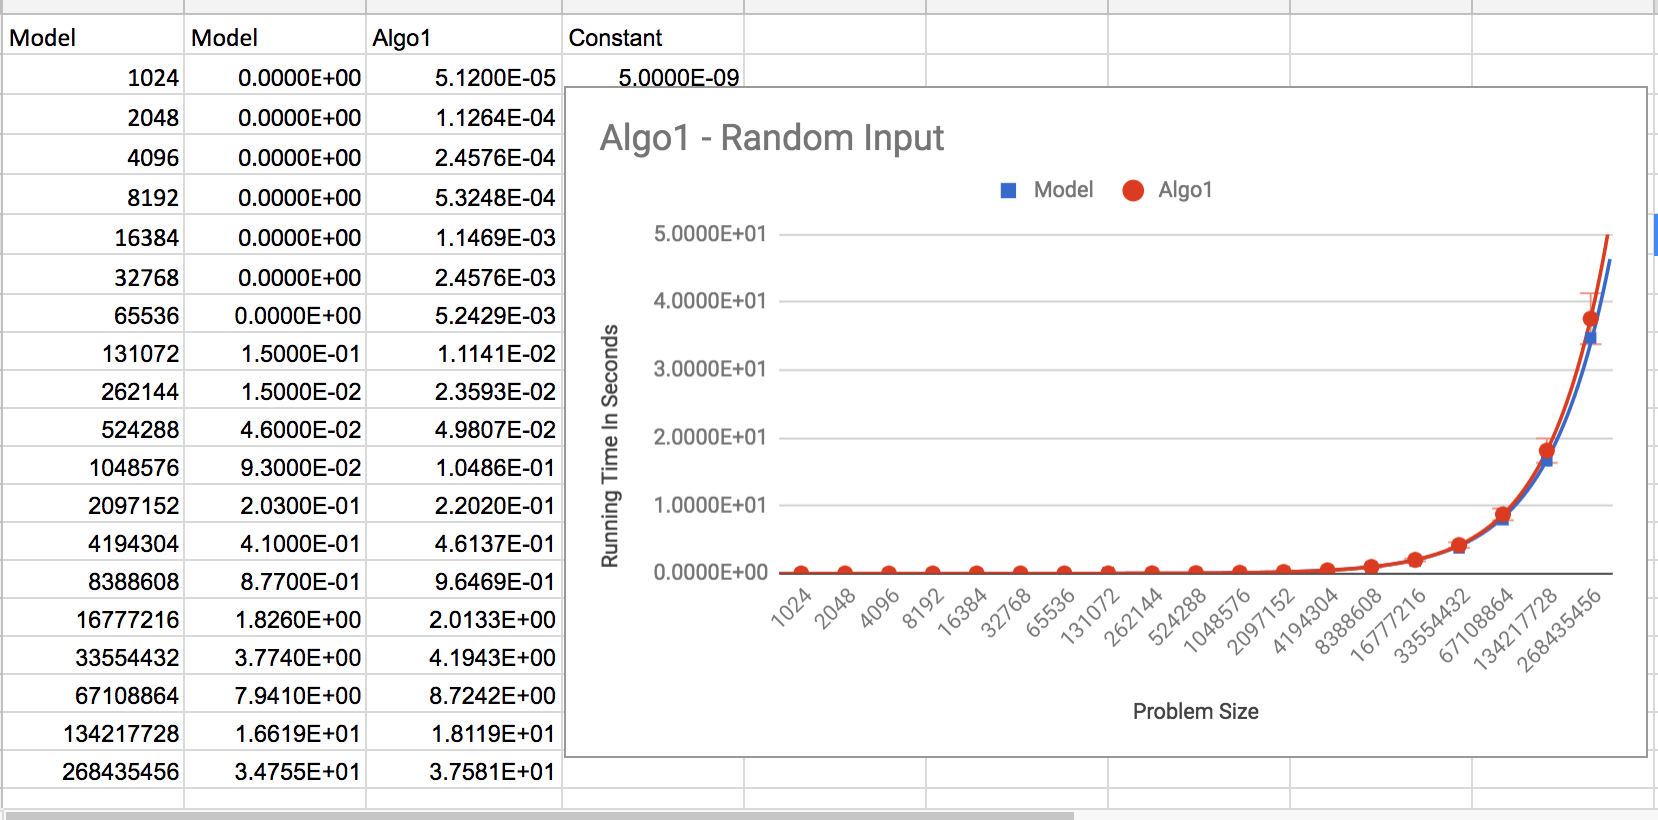
\includegraphics[height=2.5in]{./part3_algo1.jpeg}}

     %%%%%%%%%%%%%%%%%%%%%%%%%%%%%%%%%%%%%%%%%%%%%%%%%%%%%%%
     % enter your constant value and replace the image below
     %%%%%%%%%%%%%%%%%%%%%%%%%%%%%%%%%%%%%%%%%%%%%%%%%%%%%%%

      Algo 2: $T(N) =\Theta(\ \fbox{\color{black}{Your function}}\ )$
      \hfill Your constant =  \fbox{\color{black}{Your value}}

     \centerline{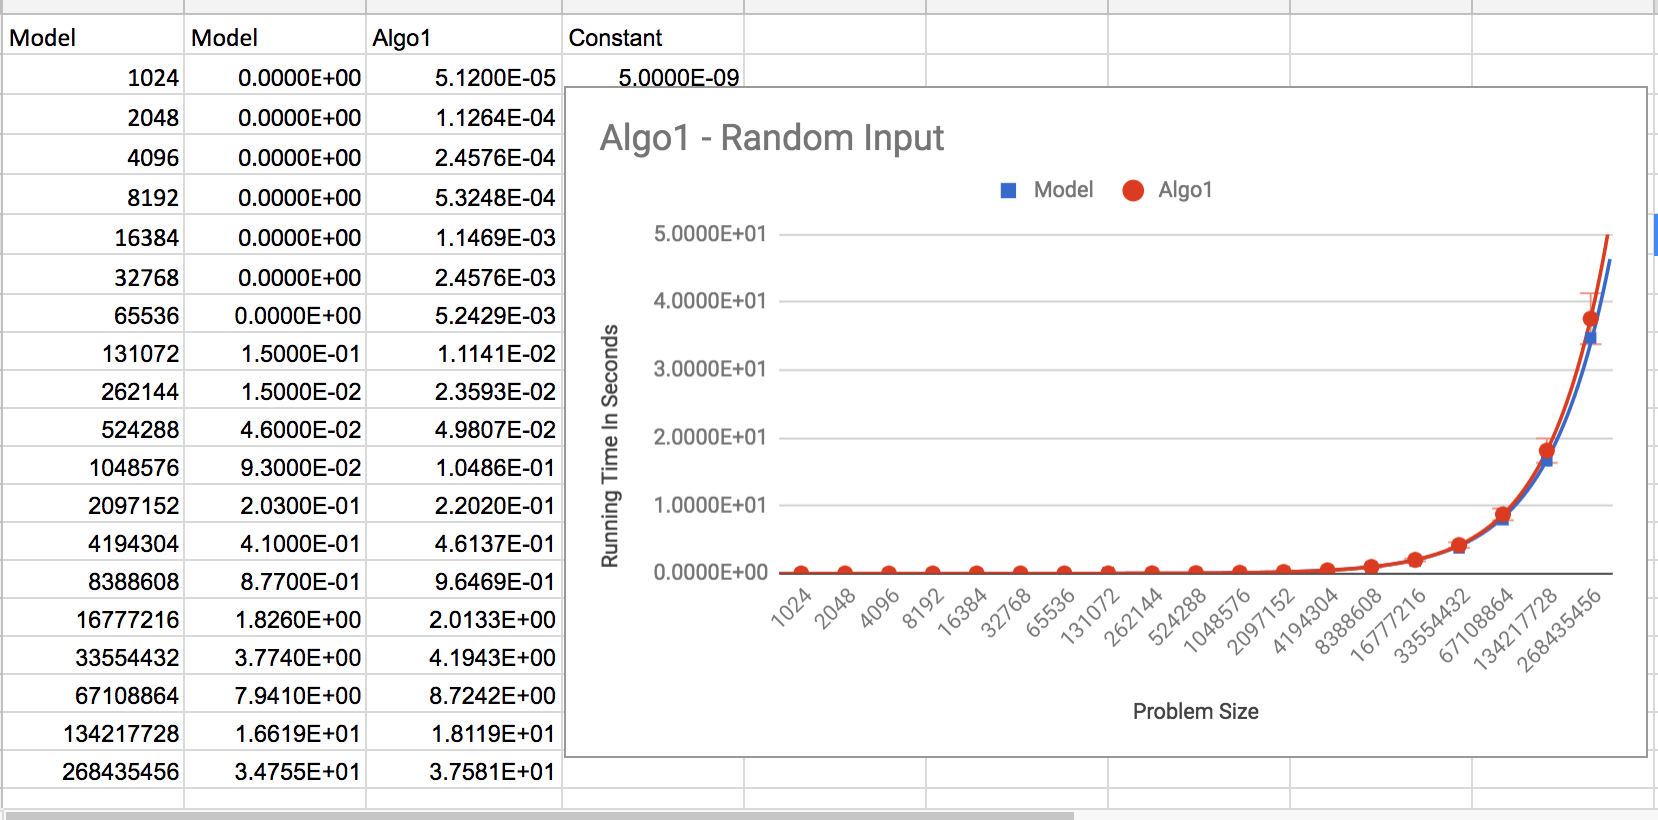
\includegraphics[height=2.5in]{./part3_algo1.jpeg}}

     %%%%%%%%%%%%%%%%%%%%%%%%%%%%%%%%%%%%%%%%%%%%%%%%%%%%%%%
     % enter your constant value and replace the image below
     %%%%%%%%%%%%%%%%%%%%%%%%%%%%%%%%%%%%%%%%%%%%%%%%%%%%%%%

      Algo 3: $T(N) =\Theta(\ \fbox{\color{black}{Your function}}\ )$
      \hfill Your constant =  \fbox{\color{black}{Your value}}

     \centerline{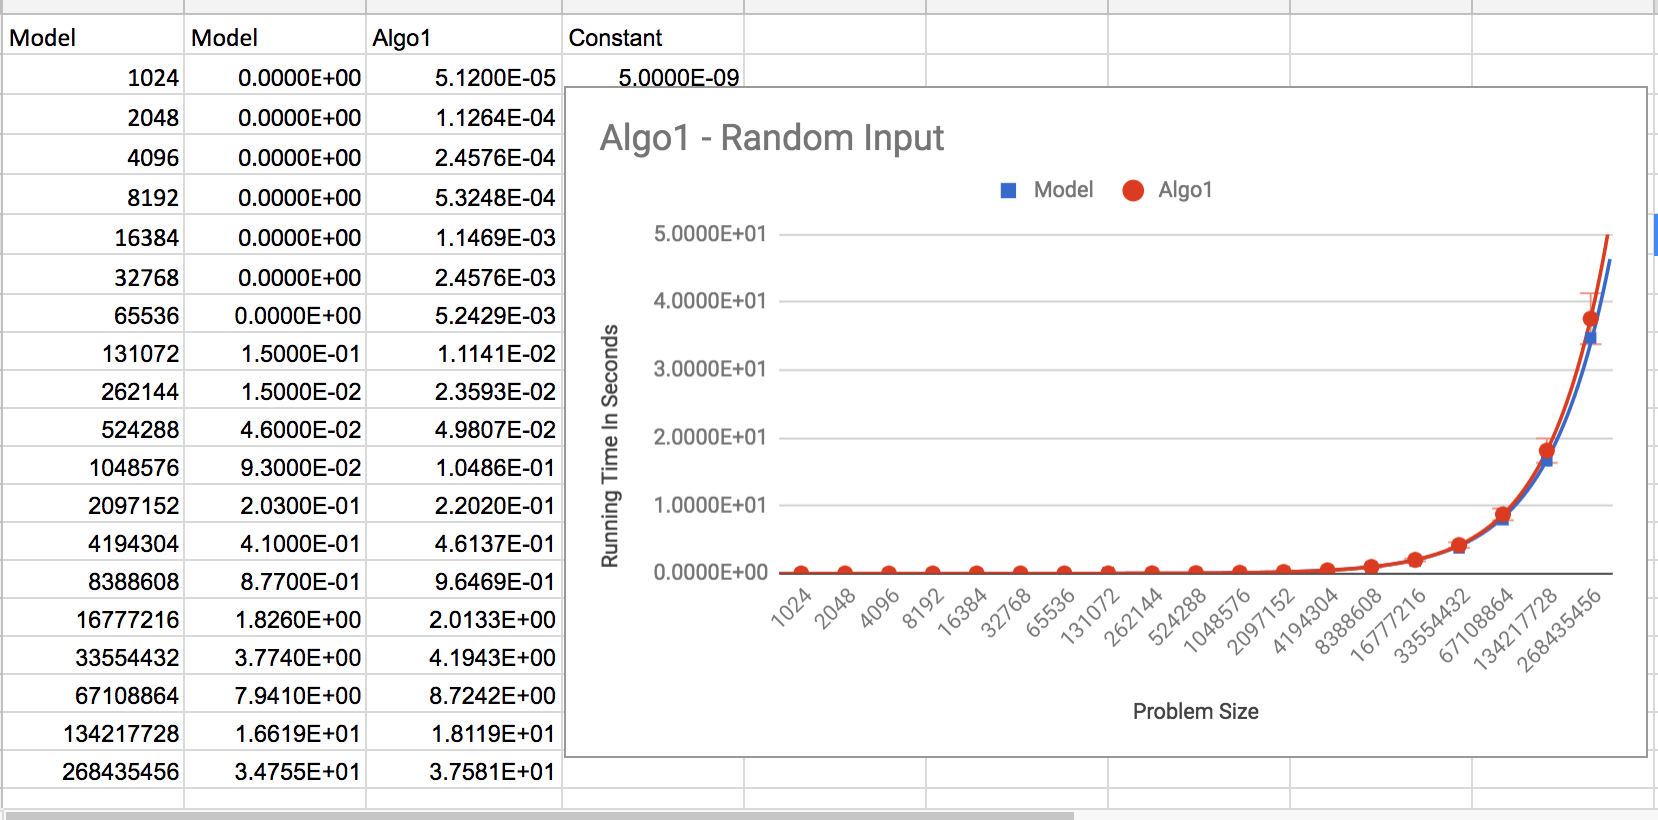
\includegraphics[height=2.5in]{./part3_algo1.jpeg}}

     \newpage



 Your answer for this part will be split into:
 \begin{enumerate}
 \item your submitted {\tt A8.java} file,
 \item your submitted {\tt part3.xlsx} file, and
 \item your three constant values and three figures on the previous page.
 \end{enumerate}

 Finally, here are some questions for you to think about before moving on to the
 next part:

 \begin{itemize}
     \item Do the three algorithms have the same order of growth on random
     inputs?
     \item Can you rank them in order of most to least efficient on random
     inputs?
     \item What is the unit for the constant values you chose? Do you understand
     their magnitude?
   \end{itemize}
 }

  %%%%%%%%%%%%%%%%%%%%%%%%%%%%%%%%%%%%%%%%%%%%%%%%%%%%%%%%%%%%%%%%%%%%%%%%%%%
   \item                            % Part 4
  %%%%%%%%%%%%%%%%%%%%%%%%%%%%%%%%%%%%%%%%%%%%%%%%%%%%%%%%%%%%%%%%%%%%%%%%%%%
   {\bf \color{red} (5 points) In this part, you will study the asymptotic
   efficiency of all three sorting algorithms with already sorted inputs. The
   description of what you have to do is identical to the one for part 3 above.
   The only difference is that the input array is now fully sorted.

  Your work for this part will be done in {\tt A8.java}, in which you only
  have to complete the body of the method called {\tt part4}. You may not
  modify any other code for this part.

 Your answer for this part will be split into:
 \begin{enumerate}
 \item your submitted {\tt A8.java} file,
 \item your submitted {\tt part4.xlsx} file, and
 \item your three constant values and three figures on the next page.
 \end{enumerate}

 Finally, here are some questions for you to think about before moving on to the
 next part:

 \begin{itemize}
     \item Do the three algorithms have the same order of growth on sorted
     inputs?
     \item Can you rank them in order of most to least efficient on sorted
     inputs?
     \item What is the unit for the constant values you chose? Do you understand
     their magnitude?
   \end{itemize}

   Make sure that all of your answers and charts for this part fit fully on the
   next page. Of course, all chart titles will have to be updated to``sorted
   input" instead of ``random input".

   \newpage

   %%%%%%%%%%%%%%%%%%%%%%%%%%%%%%%%%%%%%%%%%%%%%%%%%%%%%%%
   % enter your constant value and replace the image below
   %%%%%%%%%%%%%%%%%%%%%%%%%%%%%%%%%%%%%%%%%%%%%%%%%%%%%%%

   Algo 1: $T(N) =\Theta(\ \fbox{\color{black}{Your function}}\ )$
   \hfill Your constant =  \fbox{\color{black}{Your value}}

   \centerline{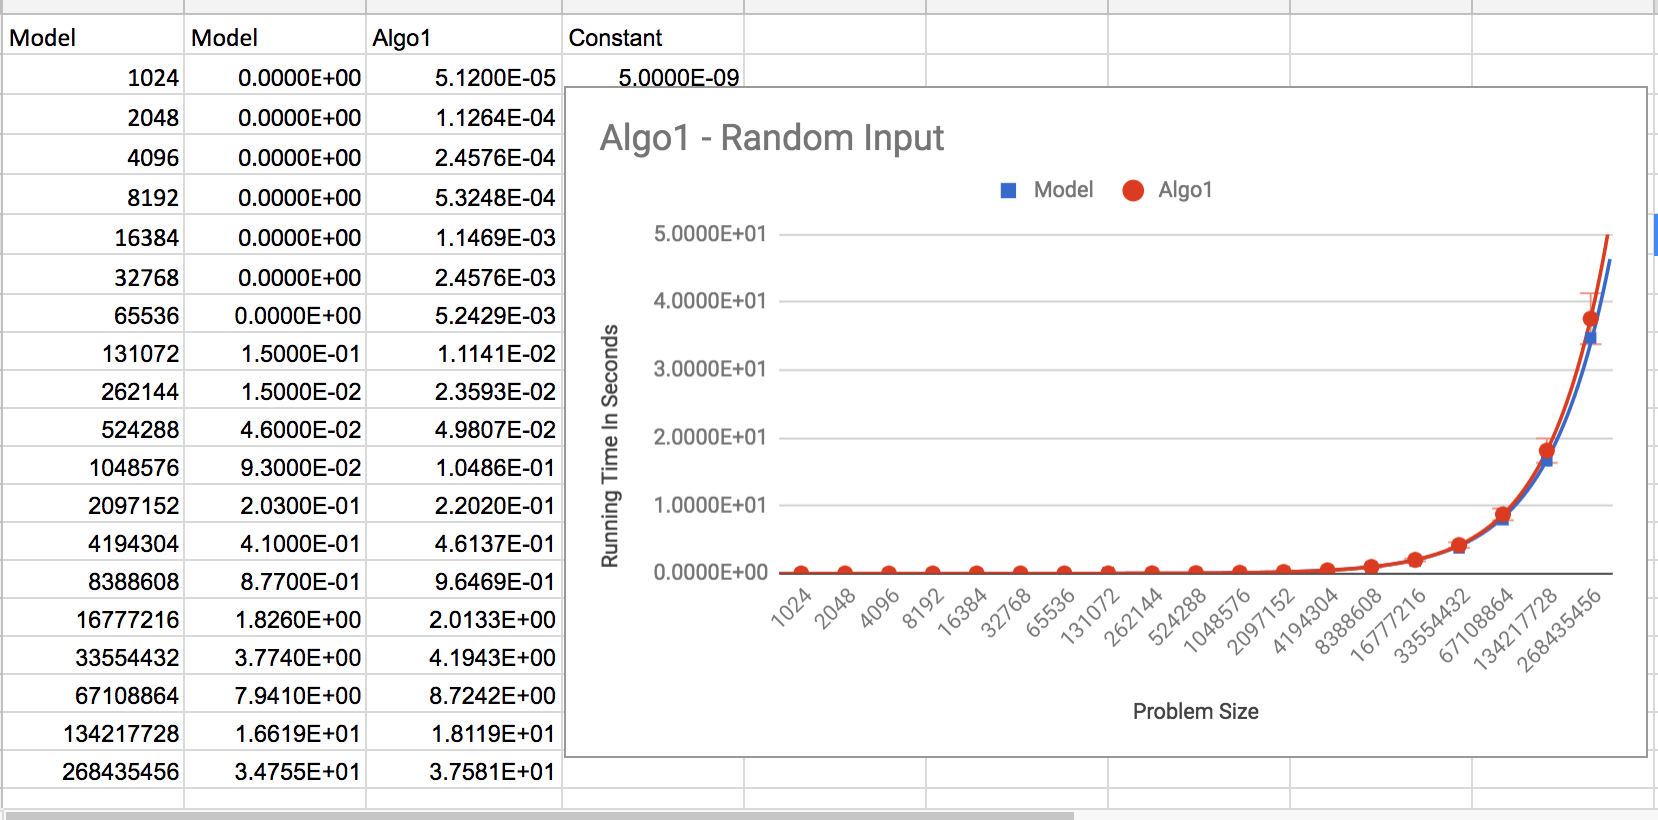
\includegraphics[height=2.5in]{./part3_algo1.jpeg}}

   %%%%%%%%%%%%%%%%%%%%%%%%%%%%%%%%%%%%%%%%%%%%%%%%%%%%%%%
   % enter your constant value and replace the image below
   %%%%%%%%%%%%%%%%%%%%%%%%%%%%%%%%%%%%%%%%%%%%%%%%%%%%%%%

    Algo 2: $T(N) =\Theta(\ \fbox{\color{black}{Your function}}\ )$
    \hfill Your constant =  \fbox{\color{black}{Your value}}

   \centerline{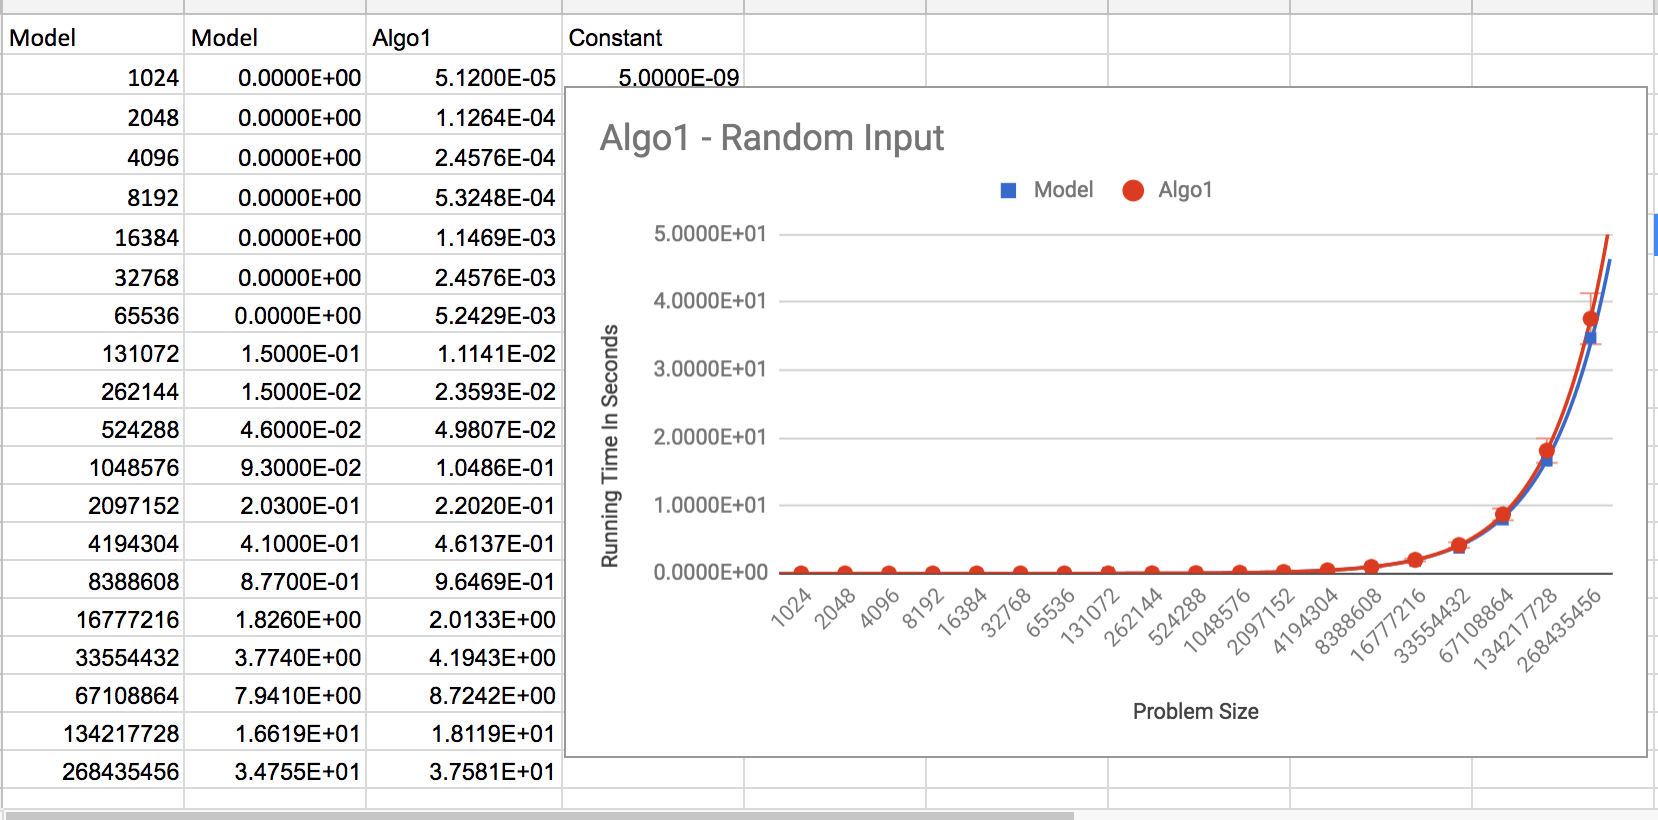
\includegraphics[height=2.5in]{./part3_algo1.jpeg}}

   %%%%%%%%%%%%%%%%%%%%%%%%%%%%%%%%%%%%%%%%%%%%%%%%%%%%%%%
   % enter your constant value and replace the image below
   %%%%%%%%%%%%%%%%%%%%%%%%%%%%%%%%%%%%%%%%%%%%%%%%%%%%%%%

    Algo 3: $T(N) =\Theta(\ \fbox{\color{black}{Your function}}\ )$
    \hfill Your constant =  \fbox{\color{black}{Your value}}

   \centerline{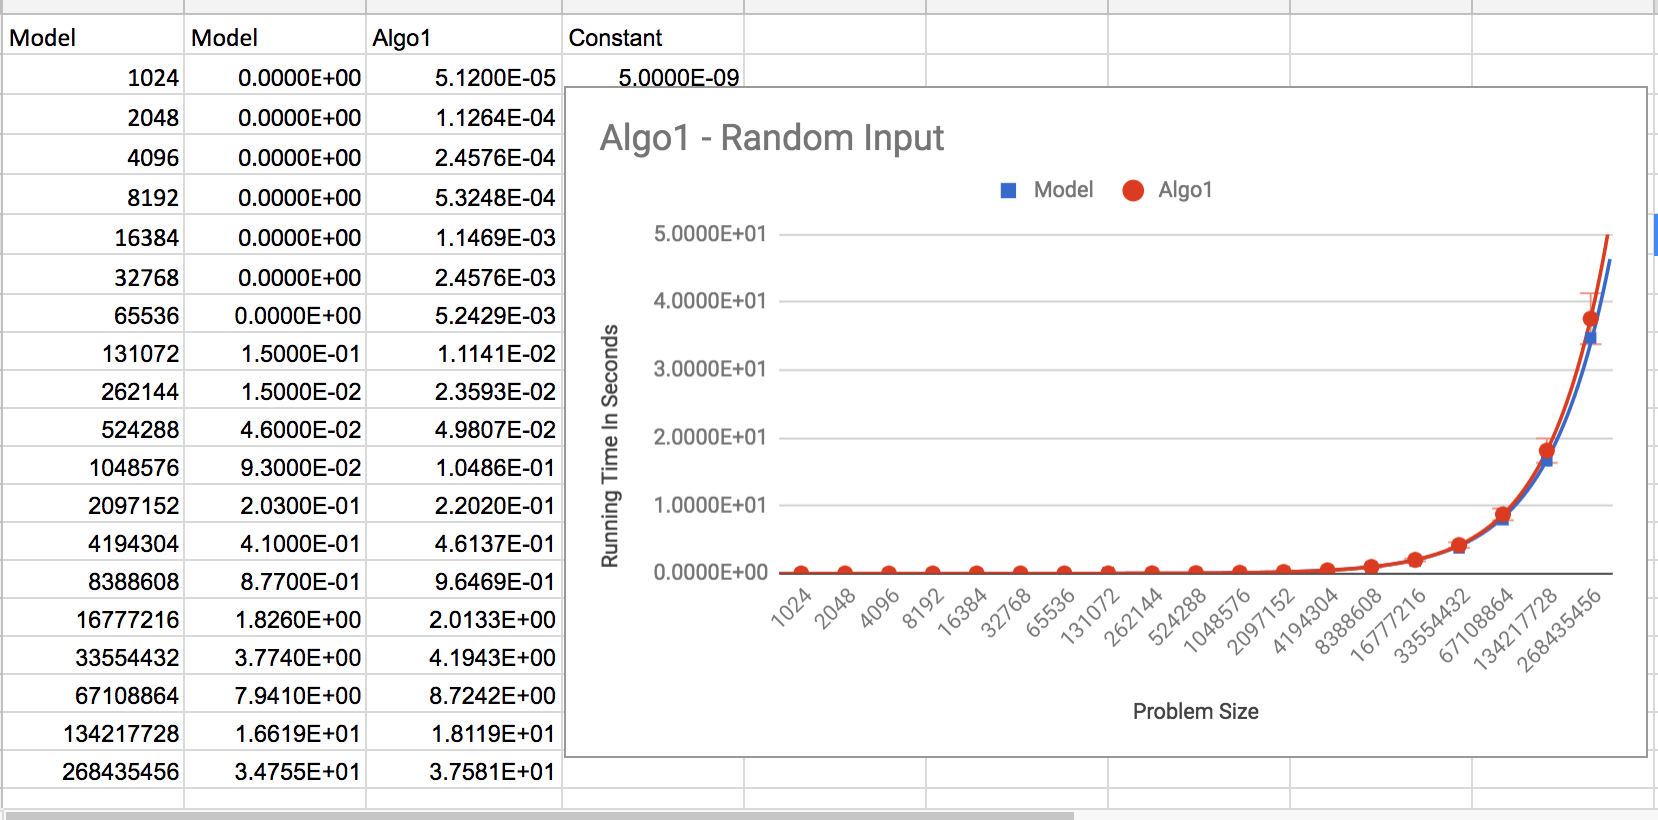
\includegraphics[height=2.5in]{./part3_algo1.jpeg}}
}
   \newpage


  %%%%%%%%%%%%%%%%%%%%%%%%%%%%%%%%%%%%%%%%%%%%%%%%%%%%%%%%%%%%%%%%%%%%%%%%%%%
   \item                            % Part 5
  %%%%%%%%%%%%%%%%%%%%%%%%%%%%%%%%%%%%%%%%%%%%%%%%%%%%%%%%%%%%%%%%%%%%%%%%%%%
   {\bf \color{red} (5 points) In this part, you will study the asymptotic
   efficiency of all three sorting algorithms with inputs that are sorted in
   reverse order. The description of what you have to do is identical to the one
   for part 3 above. The only difference is that the input array is now fully
   sorted in reverse order.

  Your work for this part will be done in {\tt A8.java}, in which you only
  have to complete the body of the method called {\tt part5}. You may not
  modify any other code for this part.

 Your answer for this part will be split into:
 \begin{enumerate}
 \item your submitted {\tt A8.java} file,
 \item your submitted {\tt part5.xlsx} file, and
 \item your three constant values and three figures on the next page.
 \end{enumerate}

 Finally, here are some questions for you to think about before moving on to the
 next part:

 \begin{itemize}
     \item Do the three algorithms have the same order of growth on
     reverse-sorted inputs?
     \item Can you rank them in order of most to least efficient on
     reverse-sorted inputs?
     \item What is the unit for the constant values you chose? Do you understand
     their magnitude?
   \end{itemize}

   Make sure that all of your answers and charts for this part fit fully on the
   next page. Of course, all chart titles will have to be updated to
  ``reverse-sorted input".

   \newpage

   %%%%%%%%%%%%%%%%%%%%%%%%%%%%%%%%%%%%%%%%%%%%%%%%%%%%%%%
   % enter your constant value and replace the image below
   %%%%%%%%%%%%%%%%%%%%%%%%%%%%%%%%%%%%%%%%%%%%%%%%%%%%%%%

   Algo 1: $T(N) =\Theta(\ \fbox{\color{black}{Your function}}\ )$
   \hfill Your constant =  \fbox{\color{black}{Your value}}

   \centerline{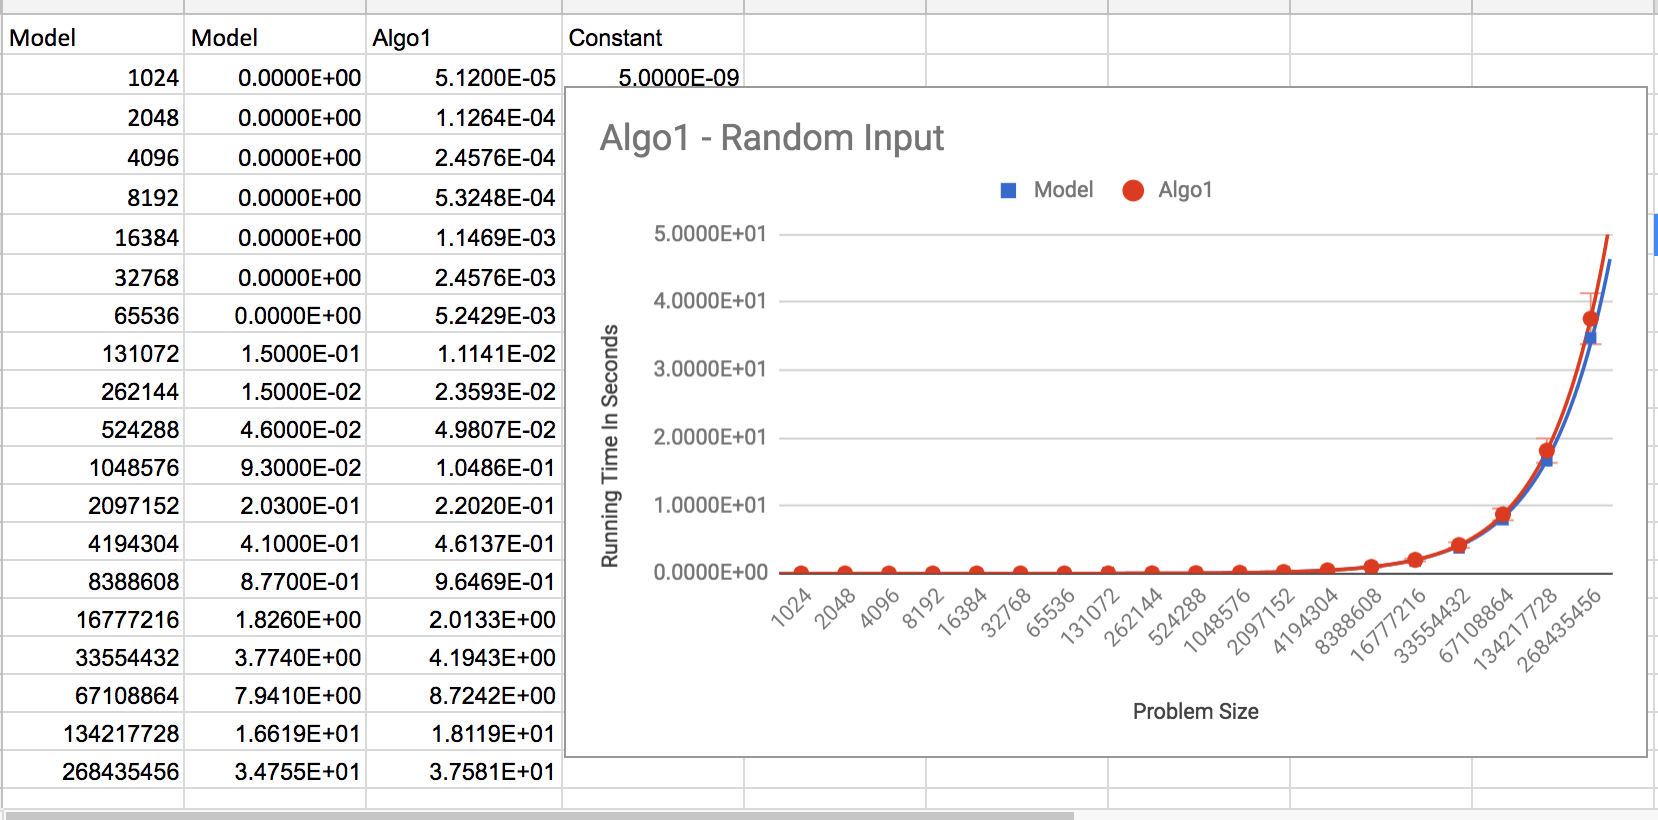
\includegraphics[height=2.5in]{./part3_algo1.jpeg}}

   %%%%%%%%%%%%%%%%%%%%%%%%%%%%%%%%%%%%%%%%%%%%%%%%%%%%%%%
   % enter your constant value and replace the image below
   %%%%%%%%%%%%%%%%%%%%%%%%%%%%%%%%%%%%%%%%%%%%%%%%%%%%%%%

    Algo 2: $T(N) =\Theta(\ \fbox{\color{black}{Your function}}\ )$
    \hfill Your constant =  \fbox{\color{black}{Your value}}

   \centerline{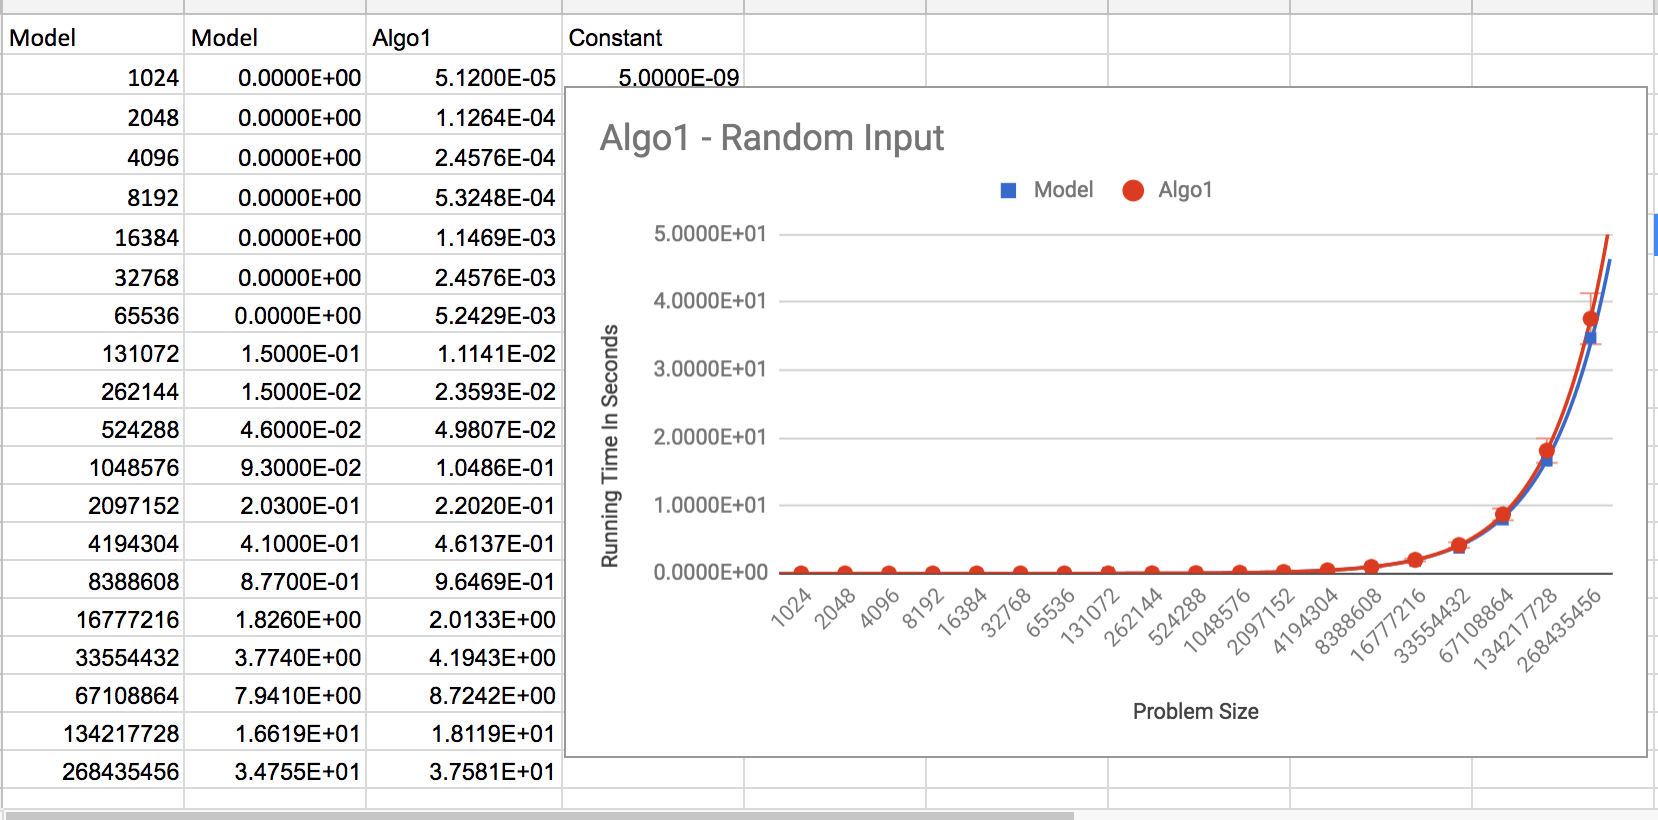
\includegraphics[height=2.5in]{./part3_algo1.jpeg}}

   %%%%%%%%%%%%%%%%%%%%%%%%%%%%%%%%%%%%%%%%%%%%%%%%%%%%%%%
   % enter your constant value and replace the image below
   %%%%%%%%%%%%%%%%%%%%%%%%%%%%%%%%%%%%%%%%%%%%%%%%%%%%%%%

    Algo 3: $T(N) =\Theta(\ \fbox{\color{black}{Your function}}\ )$
    \hfill Your constant =  \fbox{\color{black}{Your value}}

   \centerline{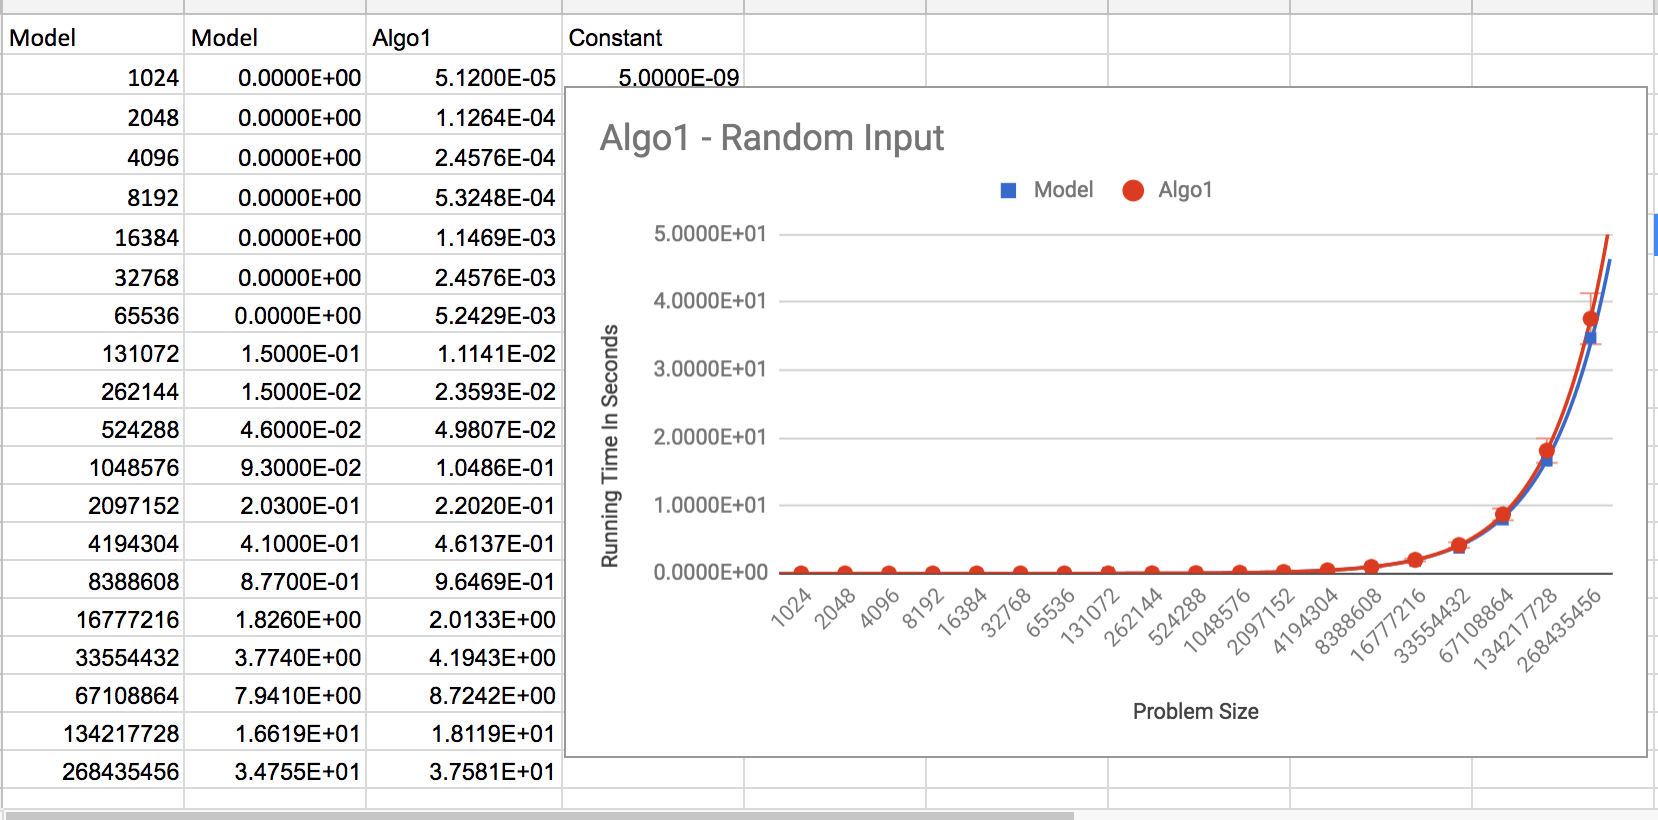
\includegraphics[height=2.5in]{./part3_algo1.jpeg}}

   \newpage
}

  %%%%%%%%%%%%%%%%%%%%%%%%%%%%%%%%%%%%%%%%%%%%%%%%%%%%%%%%%%%%%%%%%%%%%%%%%%%
   \item                            % Part 6
  %%%%%%%%%%%%%%%%%%%%%%%%%%%%%%%%%%%%%%%%%%%%%%%%%%%%%%%%%%%%%%%%%%%%%%%%%%%
   {\bf \color{red} (5 points) In this part, you will study the asymptotic
   efficiency of all three sorting algorithms with input arrays whose elements
   are all equal. The description of what you have to do is identical to the one
   for part 3 above. The only difference is that the input array is now filled
   with the value 1.

  Your work for this part will be done in {\tt A8.java}, in which you only
  have to complete the body of the method called {\tt part6}. You may not
  modify any other code for this part.

 Your answer for this part will be split into:
 \begin{enumerate}
 \item your submitted {\tt A8.java} file,
 \item your submitted {\tt part6.xlsx} file, and
 \item your three constant values and three figures on the next page.
 \end{enumerate}

 Finally, here are some questions for you to think about before moving on to the
 next part:

 \begin{itemize}
     \item Do the three algorithms have the same order of growth on
     equal-value inputs?
     \item Can you rank them in order of most to least efficient on
     equal-value inputs?
     \item What is the unit for the constant values you chose? Do you understand
     their magnitude?
   \end{itemize}

   Make sure that all of your answers and charts for this part fit fully on the
   next page. Of course, all chart titles will have to be updated to
  ``equal-value input".

   \newpage

   %%%%%%%%%%%%%%%%%%%%%%%%%%%%%%%%%%%%%%%%%%%%%%%%%%%%%%%
   % enter your constant value and replace the image below
   %%%%%%%%%%%%%%%%%%%%%%%%%%%%%%%%%%%%%%%%%%%%%%%%%%%%%%%

   Algo 1: $T(N) =\Theta(\ \fbox{\color{black}{Your function}}\ )$
   \hfill Your constant =  \fbox{\color{black}{Your value}}

   \centerline{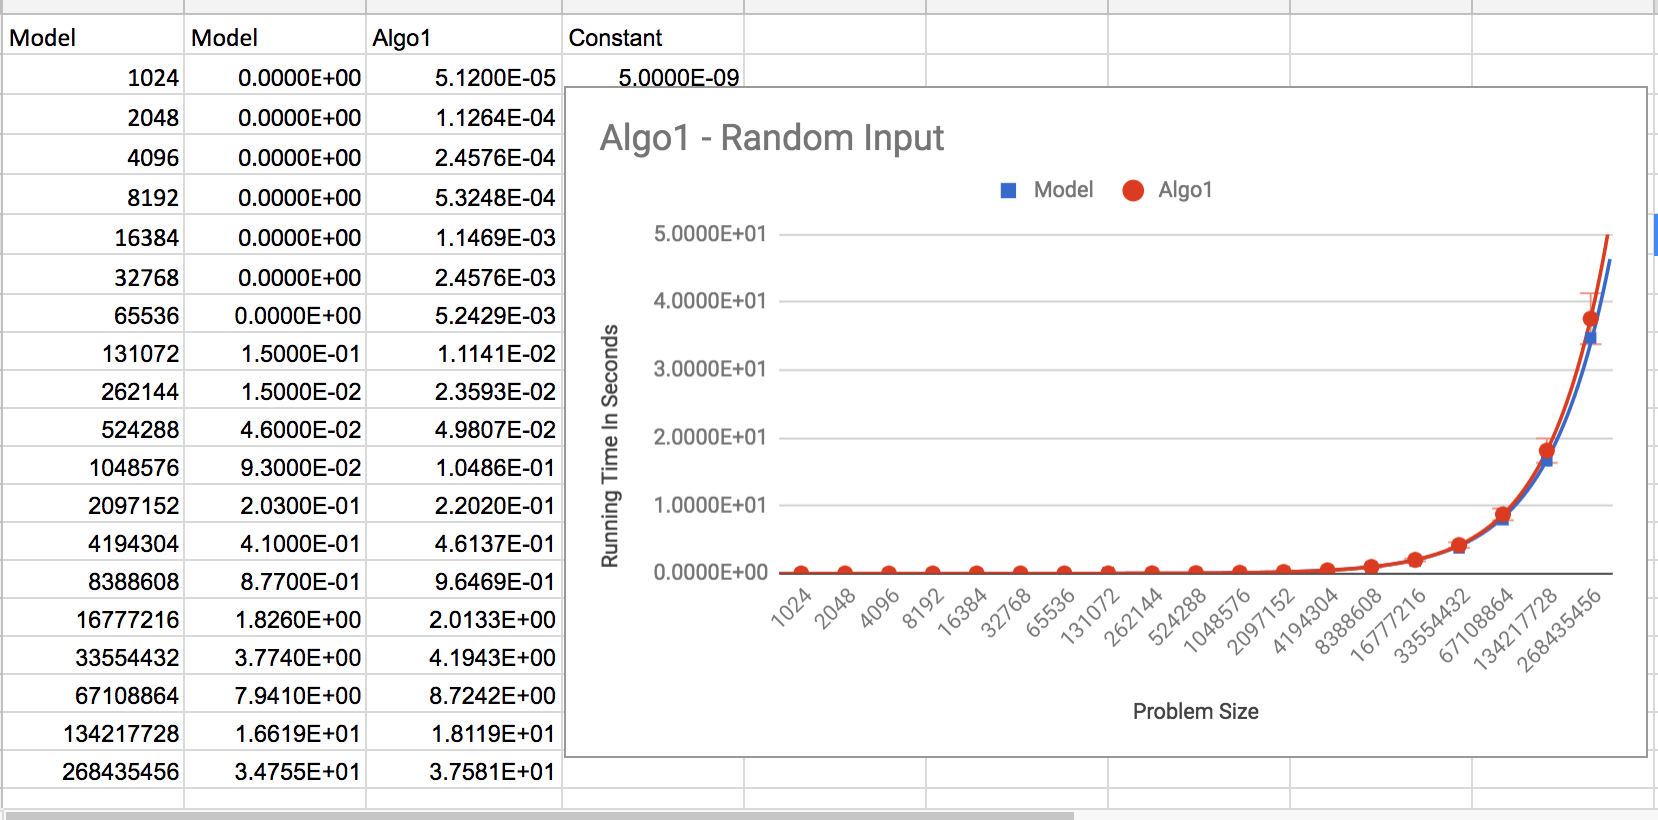
\includegraphics[height=2.5in]{./part3_algo1.jpeg}}

   %%%%%%%%%%%%%%%%%%%%%%%%%%%%%%%%%%%%%%%%%%%%%%%%%%%%%%%
   % enter your constant value and replace the image below
   %%%%%%%%%%%%%%%%%%%%%%%%%%%%%%%%%%%%%%%%%%%%%%%%%%%%%%%

    Algo 2: $T(N) =\Theta(\ \fbox{\color{black}{Your function}}\ )$
    \hfill Your constant =  \fbox{\color{black}{Your value}}

   \centerline{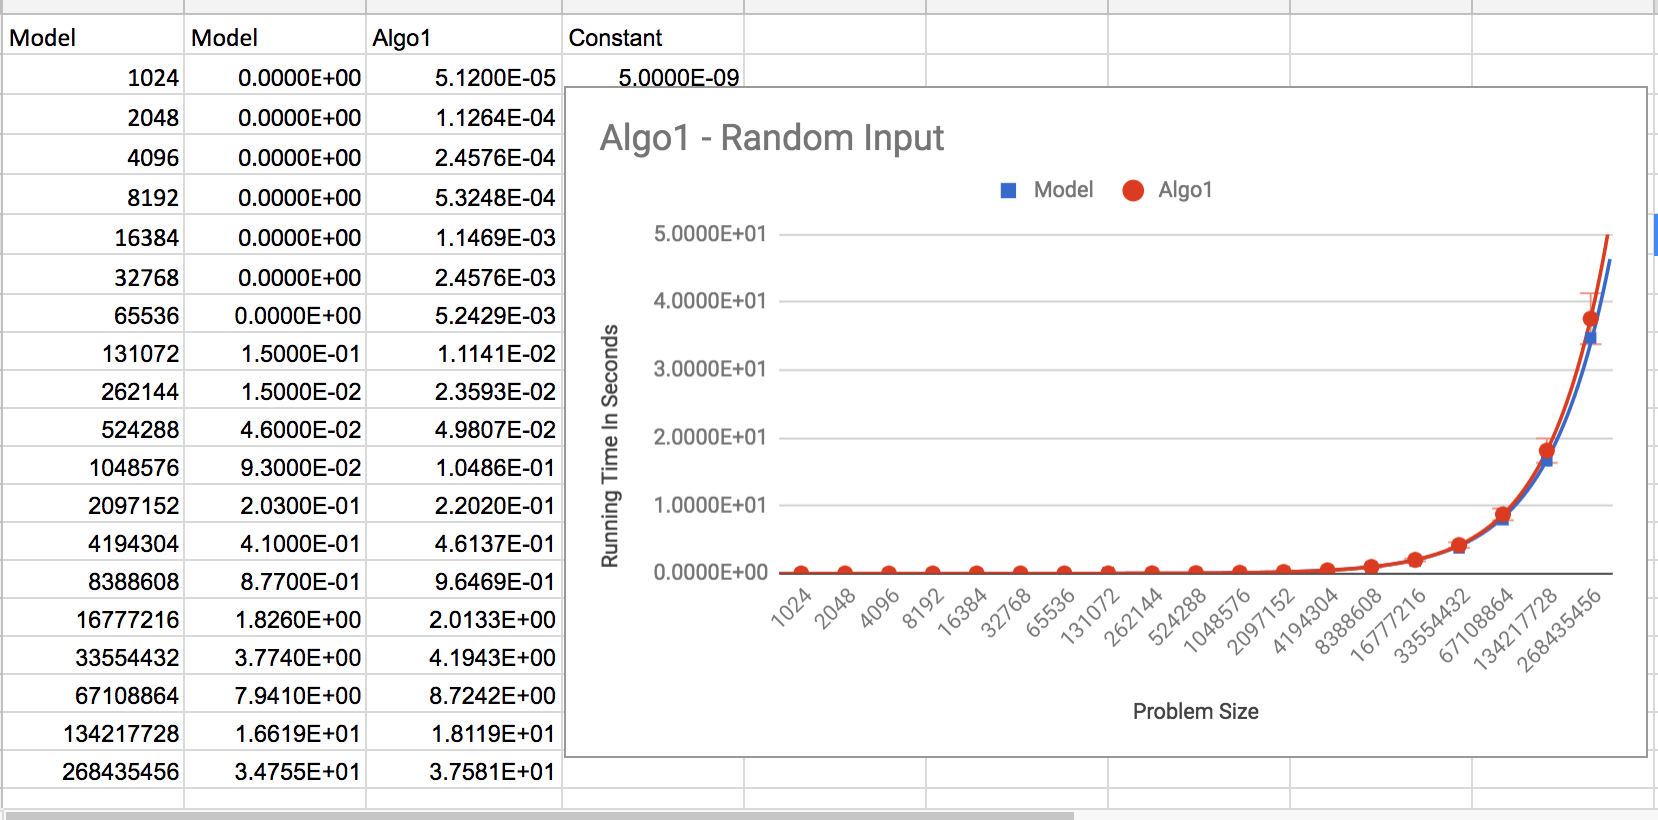
\includegraphics[height=2.5in]{./part3_algo1.jpeg}}

   %%%%%%%%%%%%%%%%%%%%%%%%%%%%%%%%%%%%%%%%%%%%%%%%%%%%%%%
   % enter your constant value and replace the image below
   %%%%%%%%%%%%%%%%%%%%%%%%%%%%%%%%%%%%%%%%%%%%%%%%%%%%%%%
ion
    Algo 3: $T(N) =\Theta(\ \fbox{\color{black}{Your function}}\ )$
    \hfill Your constant =  \fbox{\color{black}{Your value}}

   \centerline{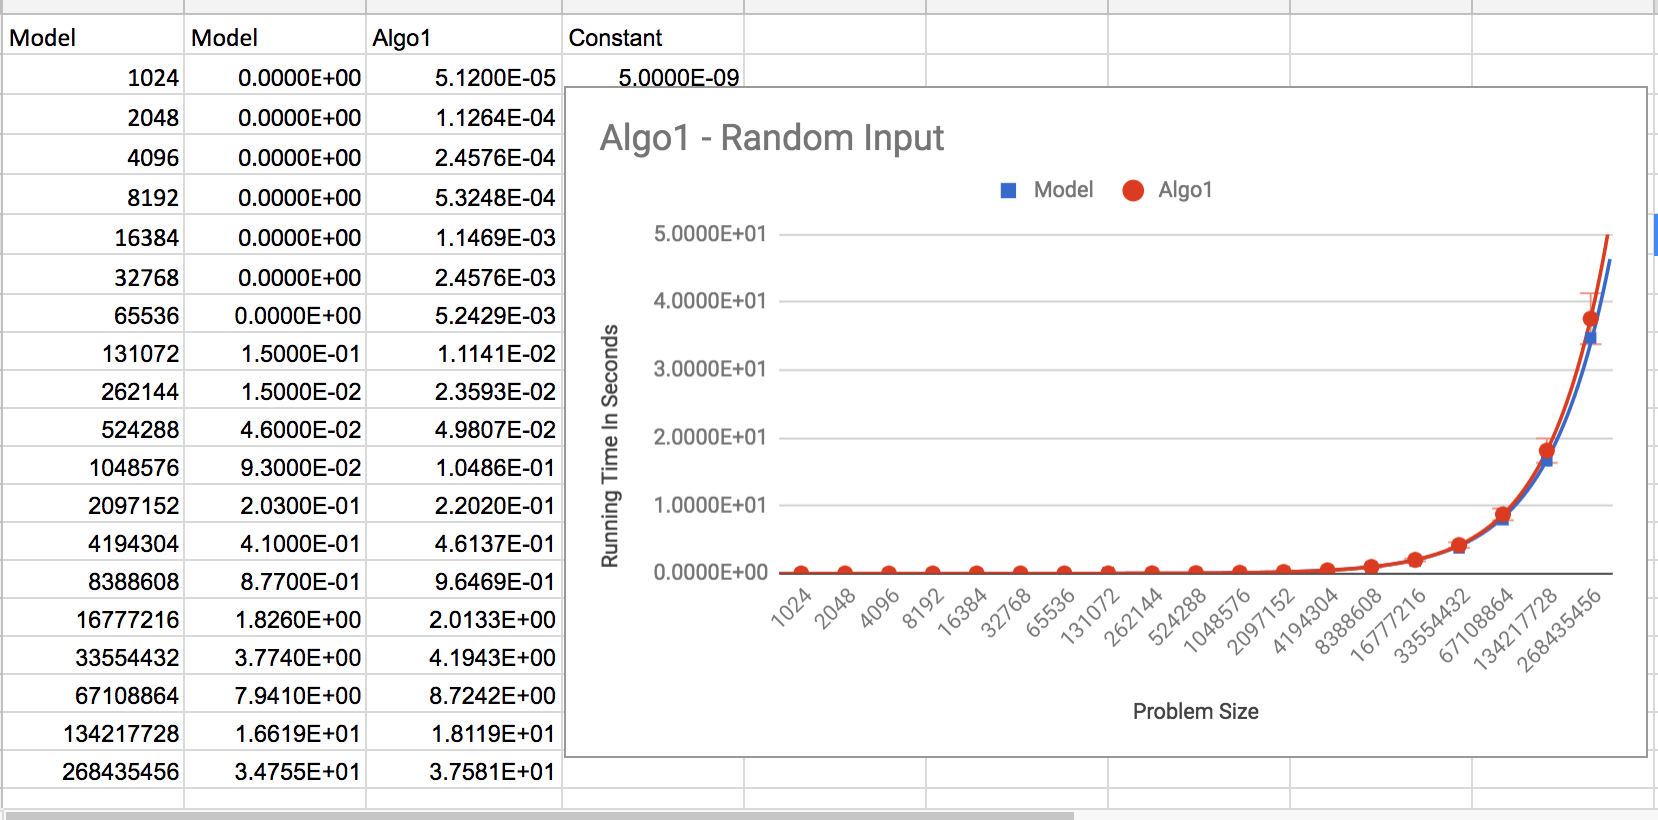
\includegraphics[height=2.5in]{./part3_algo1.jpeg}}

   \newpage
 }


  %%%%%%%%%%%%%%%%%%%%%%%%%%%%%%%%%%%%%%%%%%%%%%%%%%%%%%%%%%%%%%%%%%%%%%%%%%%
   \item                            % Part 7
  %%%%%%%%%%%%%%%%%%%%%%%%%%%%%%%%%%%%%%%%%%%%%%%%%%%%%%%%%%%%%%%%%%%%%%%%%%%
   {\bf \color{red} (5 points) In this part, you will NOT study the asymptotic
   efficiency of the algorithms. Instead, you will study how their
   running time varies with the level of "sortedness" of the input array.
   More precisely, you will run each algorithm on a fixed-size array, namely
   $2^{20}$ elements. Starting from a fully sorted array (in increasing order),
   you will increase the number of elements that are swapped using the
   {\tt Rand.shuffleArray} method with values of $n$ (the third argument)
   ranging from 0 ro 5,000, in increments of 100, for a total number of 51
   runs for each algorithm.

   The output of your program will be the values of $n$ and the corresponding
   running times in seconds. Once you have this data for all three algorithms,
   you will build an Excel workbook called {\tt part7.xlsx} containing a single
   sheet. This sheet will contain four columns of numbers, namely, from left
   to right: the value of $n$, followed by the running times for algorithms 1,
   2, and 3, in this order. To the right of these columns, you will create an
   X Y (Scatter) Chart with the value of $n$ on the $X$ axis and the running
   times on the $Y$ axis.

   This chart should follow the directions for the previous parts, with the
   following differences:
   \begin{itemize}
     \item It will contain three lines: a blue line for algorithm 1,
     an orange line for algorithm 2, and a gray line for algorithm 3. There is
     no model lines for this experiment.
     \item It will not include any markers for the data points (just a line, as
     described above).
     \item The tick marks on the $X$ axis must range from 0 to 5,000 using the
     (default) linear scale.
     \item The tick marks on the $Y$ axis must range from 0.001 to 1,000 using
     a {\bf logarithmic} scale in base 10.
     \item The tick labels for the $X$ axis must appear at the bottom of the
     chart, whereas the tick labels for the $Y$ axis must appear at the left of
     the chart.
     \item The title of the chart must be "FROM SORTED TO RANDOM".
   \end{itemize}

  Your work for this part will be done in {\tt A8.java}, in which you only
  have to complete the body of the method called {\tt part7}. You may not
  modify any other code for this part.

 Your answer for this part will be split into:
 \begin{enumerate}
 \item your submitted {\tt A8.java} file,
 \item your submitted {\tt part7.xlsx} file, and
 \item the figure on the next page.
 \end{enumerate}

   \newpage

   %%%%%%%%%%%%%%%%%%%%%%%%%%%%%%%%%%%%%%%%%%%%%%%%%%%%%%%
   % replace the image below
   %%%%%%%%%%%%%%%%%%%%%%%%%%%%%%%%%%%%%%%%%%%%%%%%%%%%%%%

   \centerline{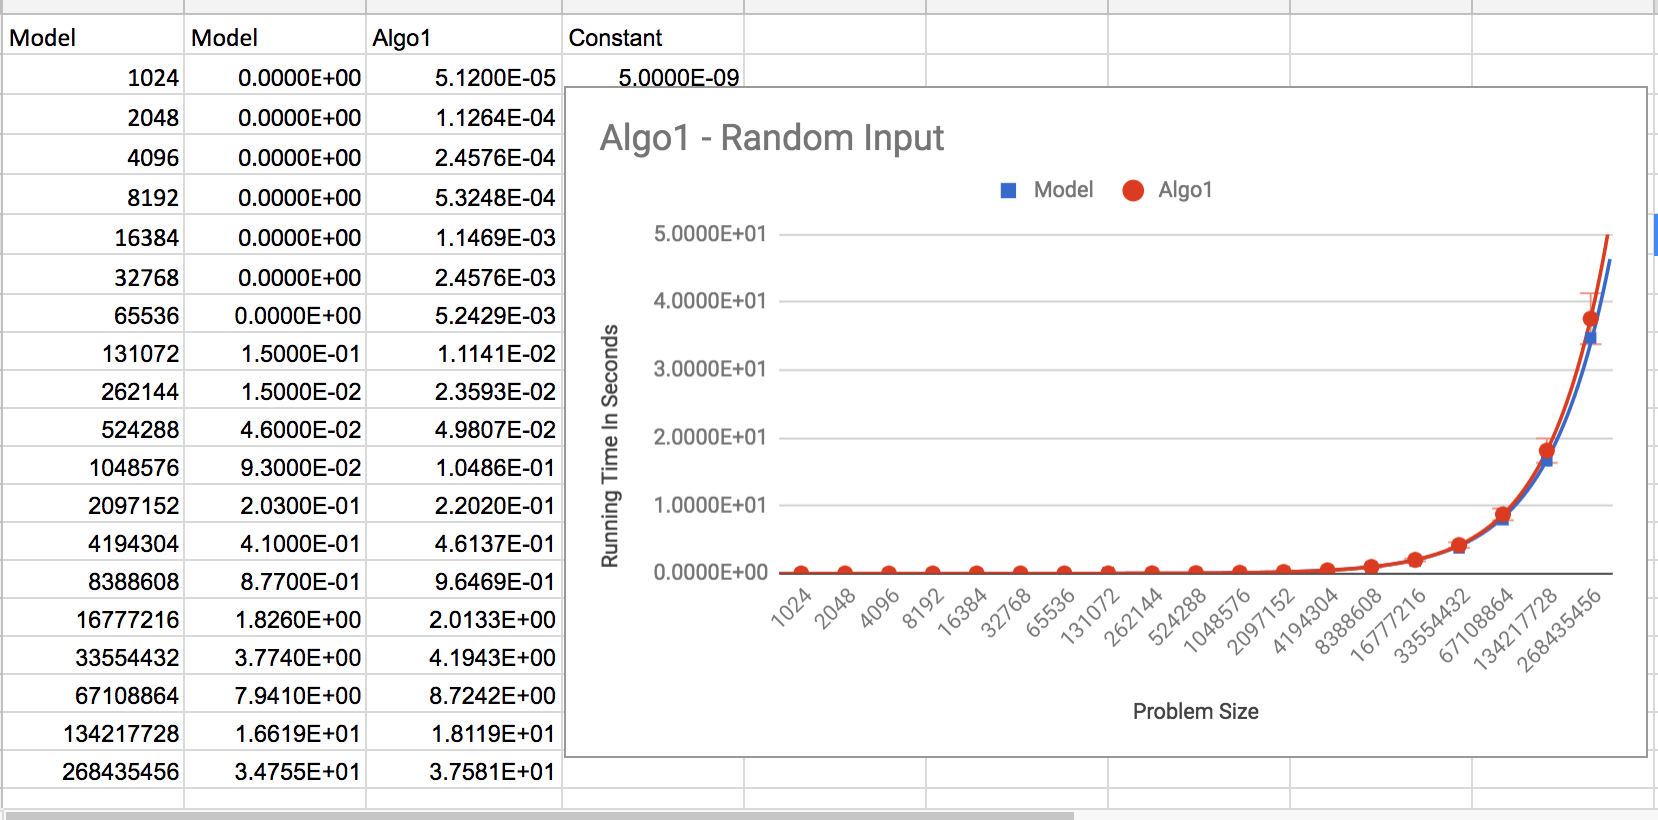
\includegraphics[height=2.5in]{./part3_algo1.jpeg}}
 }

  %%%%%%%%%%%%%%%%%%%%%%%%%%%%%%%%%%%%%%%%%%%%%%%%%%%%%%%%%%%%%%%%%%%%%%%%%%%
   \item                            % Part 8
  %%%%%%%%%%%%%%%%%%%%%%%%%%%%%%%%%%%%%%%%%%%%%%%%%%%%%%%%%%%%%%%%%%%%%%%%%%%
   {\bf \color{red} (5 points) The implementation of the {\tt Arrays.sort}
   method in Java 8 is rather complex. It uses quicksort at its core as well as
   other sorting algorithms in special cases. Look up the code for all of these
   methods (there is one implementation for each primitive type) and list below
   the name of all of the sorting algorithms that they use:\medskip

   Algorithm \#1 =  \fbox{\color{black}{algorithm name}}\newline

   Algorithm \#2 =  \fbox{\color{black}{algorithm name}}\newline

   Algorithm \#3 =  \fbox{\color{black}{algorithm name}}\newline

   Algorithm \#4 =  \fbox{\color{black}{algorithm name}}\newline

   Algorithm \#5 =  \fbox{\color{black}{algorithm name}}\newline

   Algorithm \#6 =  \fbox{\color{black}{algorithm name}}\newline

   Note: You may not be able to fill in all of the boxes above. Delete the boxes
   that you end up not needing, if any.
   }


  %%%%%%%%%%%%%%%%%%%%%%%%%%%%%%%%%%%%%%%%%%%%%%%%%%%%%%%%%%%%%%%%%%%%%%%%%%%
   \item                            % Part 9
  %%%%%%%%%%%%%%%%%%%%%%%%%%%%%%%%%%%%%%%%%%%%%%%%%%%%%%%%%%%%%%%%%%%%%%%%%%%
   {\bf \color{red} (5 points) After studying the implementation of the
   {\tt Arrays.sort} method for {\tt int[]}, figure out which kinds of inputs
   will force the code to use (at least once) a one-pivot quicksort.

   Once you have figured out one working pattern, complete the method called
   {\tt part9} in {\tt A8.java} that will generate the \underline{shortest
   possible array} of {\tt int}s that meets the requirement above.

   Your answer for this part will be fully contained in your submitted
   {\tt A8.java} file.

}
\end{enumerate}


\end{document}
